\section{Experiments}

\subsection{Communication Efficiency at Scale}\label{sect:experiments_square_cube}

Before we can meaningfully evaluate SWARM parallelism, we must verify our theoretical observations on communication efficiency. Here we run several controlled experiments that measure the GPU utilization and network usage for different model sizes, using the Transformer architecture~\citep{transformer} that has been widely adopted in various fields~\citep{lin2021survey}. To decouple the performance impact from other factors, we run these experiments on homogeneous V100 GPU nodes that serve one pipeline stage over the network with varying latency and bandwidth. We use a batch size of 1 and sequences of 512 tokens; the complete configuration is deferred to Appendix~\ref{appendix:detailed_setup}.


First, we measure how the model size affects the computation to communication ratio at 500 Mb/s network bandwidth in both directions. We consider 4 model configurations: the base configuration from the BERT paper~\citep{bert}, ``xxlarge" (``large'' with $d_{model}{=}4096$),  which is used in several recent works~\citep{albert,ernie3,deberta}, and a GPT-3-scale model with $d_{model}{=}12288$~\citep{gpt3}. We also evaluate a modified Transformer architecture (``Ours'') as defined in Section~\ref{sect:experiments_large} with $d_{model}{=}4096$, 3 layers per pipeline stage and 8-bit quantized activations. As we demonstrate in Appendix~\ref{appendix:compression}, this compression strategy can significantly reduce network usage with little effect on convergence. In the first three configurations, the model consists of 12 Transformer layers placed on 12 servers with a single GPU; in the last one, there are 4 servers, each hosting 3 layers.
Appendix~\ref{appendix:detailed_setup} contains FLOP and parameter counts of each configuration.




\begin{figure}[b]
\vspace{-14pt}
    \centering
    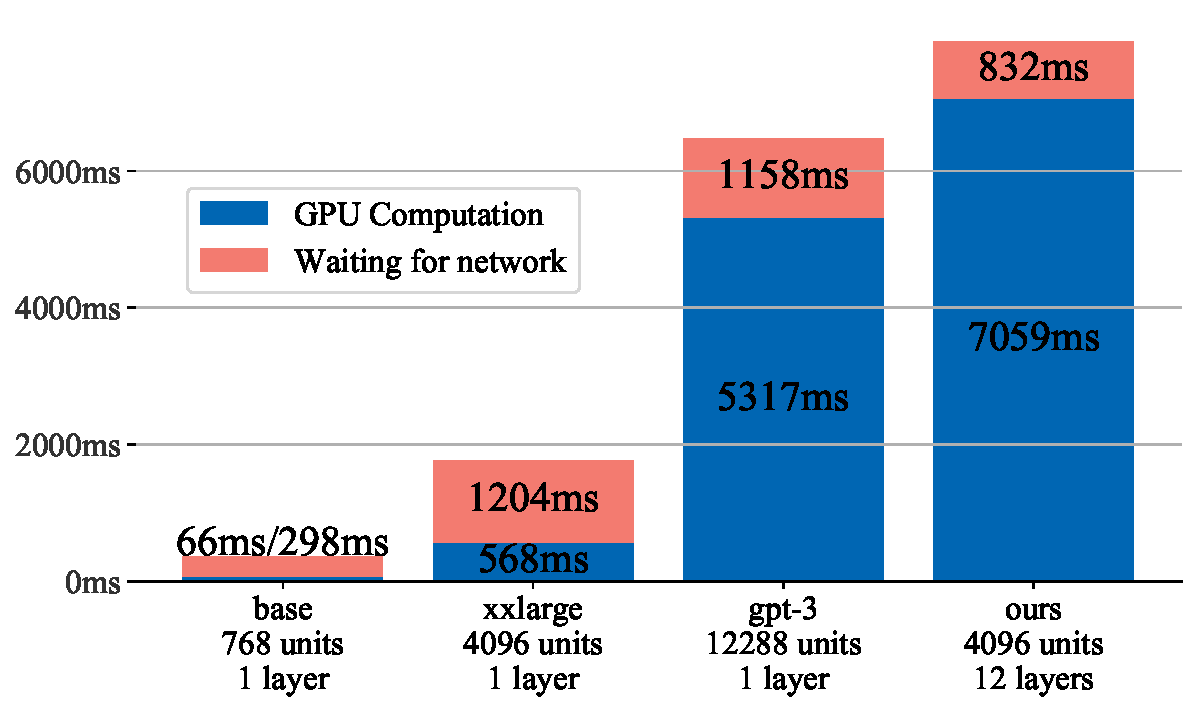
\includegraphics[width=1\linewidth]{resources/perf_absolute.pdf}
    \vspace{-12pt}
    \captionof{figure}{Pipeline computation and idle time per batch at 500 Mb/s bandwidth.}
    \label{fig:throughput_exps}
\end{figure}%
\begin{table}
    \centering
    \captionof{table}{Relative device utilization at 500 Mb/s bandwidth and varying network latency.}
    \label{tab:latency}
    \small
    \setlength{\tabcolsep}{8pt}
    \begin{tabular}[b]{@{}lcccc@{}}
    \toprule
    \multirow{2}{*}{\thead{Latency\\(RTT)}} & 
    \multicolumn{4}{c}{
    \thead{
    Relative GPU utilization\\ (100\% - idle time)
    }
    }
    
    \\
\cmidrule{2-5}                     & base & xxlarge & GPT-3 & Ours \\ \midrule
    None &   18.0\%     &  32.1\%         &  82.1\%  &  89.5\%      \\
    10ms &   11.8\%      &   28.9\%    &   79.3\%   &  87.2\%    \\
    50ms &    4.88\%      &   20.1\%    &   70.3\% &  79.5\%    \\
    100ms &    2.78\%      &    14.9\%    &  60.2\%     &   71.5\% \\
    200ms &   1.53\%     &  10.1\%    &  48.5\%   &     59.2\%    \\
    \bottomrule
    \end{tabular}
    \vspace{-6pt}
\end{table}

As depicted in Figure~\ref{fig:squarecube} (right) and Figure~\ref{fig:throughput_exps}, larger models achieve better GPU utilization rate in the same network conditions, since their communication load grows slower than computation. More importantly, even at 500 Mb/s, the resulting GPU idle time can be pushed into the 10--20\% range, either naturally for GPT-3-sized models or through activation compression for smaller models. In addition, large models maintain most of their training efficiency at the 100ms latency~(Table~\ref{tab:latency}), which is roughly equivalent to training on different continents~\citep{verizon_latency}.

\vspace{-4pt}
\subsection{Detailed Performance Comparison}\label{appendix:training_throughput}

Here we investigate how SWARM parallelism compares to existing systems for training large models: \textbf{GPipe}~\citep{huang2019gpipe} and \textbf{ZeRO-Offload}~\citep{zerooffload}.
The purpose of this section is to compare the training throughput in ``ideal'' conditions (with homogeneous reliable devices and balanced layers), as deviating from these conditions makes it \textit{infeasible} to train with baseline systems.
Still, even in such conditions the performance of different systems can vary across model architectures, and hence we want to identify the cases in which using SWARM is preferable to other approaches.
We benchmark individual SWARM components in preemptible setups in Section~\ref{sect:experiments_adaptive} and Appendix~\ref{appendix:scaling}.

We evaluate training performance for sequences of 4 Transformer layers of identical size distributed over 16 workers. Similarly to Section~\ref{sect:experiments_square_cube}, we use three layer configurations: ``xxlarge''~($d_{model} {=} 4096$, $d_{\text{FFN}} {=} 16384$, 32 heads), ``GPT-3''~($d_{model} {=} 12288$, $d_{\text{FFN}} {=} 49152$, 96 heads), and ``Ours''~($d_{model} {=} 4096$, $d_{\text{FFN}} {=} 16384$, 32 heads, 16 shared layers per block, last stage holds only the vocabulary projection layer). The microbatch size is 4 for ``xxlarge'' and 1 for ``GPT-3'' and ``Ours'', and the sequence length is 512.

To provide a more detailed view of the training performance, we measure two separate performance statistics: the training throughput and the All-Reduce time. 
The training throughput measures the rate at which the system can process training sequences, i.e., run forward and backward passes. 
More specifically, we measure the time required to process 6250 sequences of 512 tokens, which corresponds to the largest batch size used in~\citet{gpt3}.
In turn, the All-Reduce time is the time each system spends to aggregate accumulated gradients across devices. 
Intuitively, training with small batch sizes is more sensitive to the All-Reduce time (since the algorithm needs to run All-Reduce more frequently) and vice versa.


\textbf{Hardware setup:} Each worker uses a V100-PCIe GPU with 16 CPU threads (E5 v5-2660v4) and 128 GB RAM. The only exception is for ZeRO-Offload with ``GPT-3'' layers, where we had to double the RAM size because the system required 190 gigabytes at peak. Similarly to Section~\ref{sect:experiments_square_cube}, each worker can communicate at a 500 Mb/s bandwidth for both upload and download for a total of 1 Gb/s.
In terms of network latency, we consider two setups: with \textbf{no latency}, where workers communicate normally within the same rack, and with \textbf{latency}, where we introduce additional $100\pm50$ms latency directly in the kernel\footnote{More specifically, \texttt{tc qdisc add dev <...> root netem delay 100ms 50ms}}.

\textbf{GPipe configuration:} We use a popular PyTorch-based implementation of GPipe\footnote{The source code is available at \url{https://github.com/kakaobrain/torchgpipe}}. The model is partitioned into 4 stages repeated over 4 model-parallel groups. To fit into the GPU memory for the ``GPT-3'' configuration, we offload the optimizer into RAM using ZeRO-Offload. Before averaging, we use PyTorch's built-in All-Reduce to aggregate gradients.
We evaluate both the standard GPipe schedule and the 1F1B schedule~\citep{pipedream}.

\textbf{ZeRO-Offload configuration:} Each worker runs the entire model individually, then exchanges gradients with peers. For ``xxlarge'', we use the official implementation from~\cite{zerooffload}. However, for ``GPT-3'', we found that optimizer offloading still does not allow us to fit 4 layers into the GPU. For this reason, we also offload the model parameters using the \texttt{offload\_param} option.

\begin{table}
\centering
\small
\setlength{\tabcolsep}{4pt}
\captionof{table}{Training performance for different model sizes.}
\label{tab:throughput_gpt}
\begin{tabular}[b]{lcccc}
\toprule
\multirow{2}[2]{*}{System} &
  \multicolumn{2}{c}{Throughput, min/batch} &
  \multicolumn{2}{c}{All-Reduce time, min} \\ \cmidrule(lr){2-3}\cmidrule(lr){4-5} 
                 & No latency & Latency & No latency & Latency \\
 \midrule \multicolumn{5}{c}{``GPT-3'' (4 layers) }\\
 \midrule
SWARM            &  168.3 &\textbf{186.7}  &  7.4 & \textbf{7.6}   \\
GPipe            &  164.5 & 218.4 &  \multirow{2}{*}{\textbf{6.7}}    & \multirow{2}{*}{7.8}   \\
1F1B & \textbf{163.3} & 216.1 & & \\
Offload          &  272.7 & 272.7          &  25.5 & 27.3 \\
\midrule \multicolumn{5}{c}{``xxlarge'' (4 layers) }\\
\midrule
SWARM            &  44.2 & 48.2                  &  0.8  & \textbf{0.9}   \\
GPipe            &  40.1 & 108.8                  &  \multirow{2}{*}{\textbf{0.7}}  & \multirow{2}{*}{1.1}   \\
1F1B & 40.8 & 105.5 & & \\
Offload          &  \textbf{33.8} & \textbf{33.8}  &  2.8 & 4.2   \\
\midrule \multicolumn{5}{c}{Full ``Ours'' model (48 shared layers + embeddings) }\\
\midrule
SWARM            &  432.2 & 452.9                  &  0.8  &\bf 1.0   \\
GPipe            &  420.0 & 602.1                   &  \multirow{2}{*}{\bf 0.7}  & \multirow{2}{*}{1.1}   \\
1F1B             &  408.5 & 569.2 & & \\
Offload          &  \bf 372.0 &\bf 372.0  &  3.2 & 4.8   \\
\bottomrule
\end{tabular}
\vspace{-8pt}
\end{table}%

\begin{figure}[b]
\vspace{-16pt}
\centering
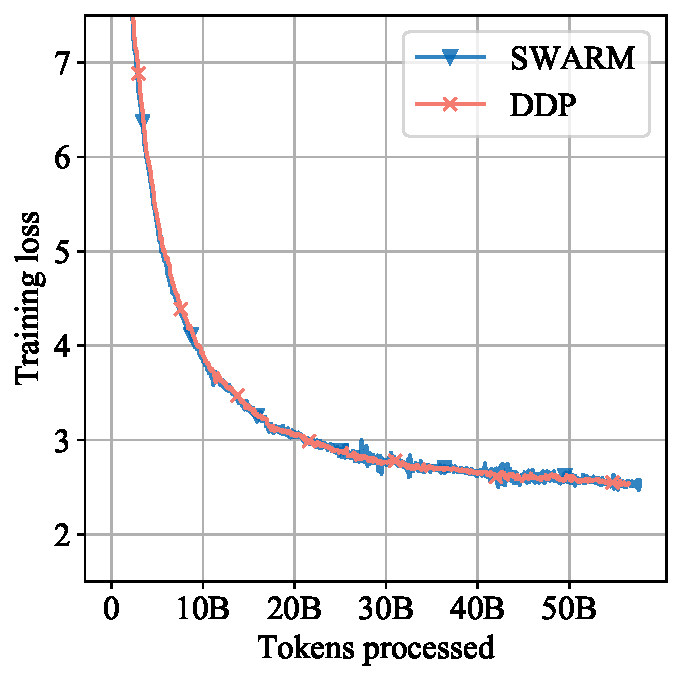
\includegraphics[ width=0.65\linewidth]{resources/learning_3stages.pdf}
\vspace{-6pt}
\captionof{figure}{Training convergence comparison.}
\label{fig:convergence}
\end{figure}

In turn, when training smaller models, ZeRO-Offload outperforms both SWARM and GPipe. This result aligns with our earlier observations in Figure~\ref{fig:squarecube}, where the same model spent most of the time waiting for the communication between pipeline stages.%

We also observe that ZeRO-Offload takes longer to aggregate gradients, likely because each peer must aggregate the entire model, whereas in SWARM and GPipe, peers aggregate a single pipeline stage. The variation between All-Reduce time in GPipe and SWARM is due to implementation differences. Overall, SWARM is competitive to HPC baselines even in an idealized homogeneous environment.

\subsection{Large-Scale Distributed Training}
\label{sect:experiments_large}

To verify the efficiency of SWARM parallelism in a practical scenario, we conduct a series of large-scale distributed experiments using preemptible (unreliable) cloud T4 and A100 GPUs over a public cloud network.

We train a Transformer language model with the architecture similar to prior work~\citep{gpt3,gptj,gptneo} and 1.01 billion parameters in total. Our model consists of 3 stages, each containing a single Transformer decoder block with $d_{model}=4096$ and 16 layers per pipeline stage. All workers within a stage serve the same group of layers, and all layers within each group use the same set of parameters, similarly to ALBERT~\citep{albert}. On top of this, the first stage also contains the embedding layer, and the last stage includes the language modeling head. Because of layer sharing, this model is equivalent to a 13B model from~\citet{gpt3} in terms of compute costs. 

We use 8-bit compression~\citep{adam8bit} for activations and gradients to reduce the communication intensity. Additional training setup details are covered in Appendix~\ref{appendix:detailed_large}.
SWARM nodes run rebalancing every $T=300$ seconds, and trainers measure peer performance using a moving average with $\alpha=0.1$. However, as we show in Section~\ref{sect:experiments_adaptive}, the throughput of SWARM is not very sensitive to the choice of these hyperparameters.



First, to verify that model parallelism with asynchronous updates does not have significant convergence issues, we train the model on the Pile~\citep{gao2020pile} dataset with 400 preemptible T4 instances, each hosting one accelerator. As a baseline, we use regular data-parallel training with offloading on 128 A100 GPUs.
We run both experiments for approximately 4 weeks and compare the learning curves.




Figure~\ref{fig:convergence} shows the results of this experiment: it can be seen that the training dynamics of two approaches are indeed similar, which demonstrates the viability of SWARM parallelism for heterogeneous and poorly-connected devices.

In the next experiment, we aim to measure the pipeline throughput in different hardware conditions and to compare it with an estimate of best-case pipeline performance.
We consider several setups: first, we use the same 400 preemptible T4 nodes; in another setup, we use 7 instances with 8 A100 GPU each; finally, we combine these fleets to create a heterogeneous setup. We examine the performance of the pipeline both with weight sharing and with standard, more common, Transformer blocks.

\begin{table}
\centering
\captionof{table}{Pipeline throughput, layer sharing.}
\label{tab:throughput}
\small
\begin{tabular}{@{}lcccc@{}}
\toprule
\multirow{2}{*}{\begin{tabular}[c]{@{}l@{}}Hardware\\ setup\end{tabular}} &
  \multicolumn{2}{c}{\begin{tabular}[c]{@{}c@{}}Throughput,\\ samples/s\end{tabular}} &
  \multicolumn{2}{c}{\begin{tabular}[c]{@{}c@{}}Optimal\\ bandwidth, Mb/s\end{tabular}} \\ \cmidrule(lr){2-3}\cmidrule(lr){4-5} 
                 & Actual & Best-case & Upload & Download \\ \midrule
T4           &  17.6      &   19.2        &   317.8     &     397.9     \\
A100          & 16.9       &   25.5        &   436.1     &     545.1     \\
T4 \& A100 &   27.3     &       ---    &   ---     &      ---    \\ \bottomrule
\end{tabular}
\end{table}
\begin{table}
\centering
\captionof{table}{Pipeline throughput, default Transformer.}
\label{tab:throughput_standard}
\small
\begin{tabular}{@{}lcc@{}}
\toprule
\multirow{2}{*}{\begin{tabular}[c]{@{}l@{}}Hardware\\ setup\end{tabular}} &
  \multicolumn{2}{c}{\begin{tabular}[c]{@{}c@{}}Throughput,\\ samples/s\end{tabular}} \\ \cmidrule(lr){2-3}
                 & Actual & Best-case \\ \midrule
T4           &  8.8      &   19.3        \\
A100          & 8.0       &   25.1        \\
T4 \& A100 &   13.4     &       ---    \\ \bottomrule
\end{tabular}
\end{table}






We measure the number of randomly generated samples processed by the pipeline both in our infrastructure and the ideal case that ignores all network-related operations (i.e., has infinite bandwidth and zero latency). The ideal case is emulated by executing a single pipeline stage 3 times locally on a single server and multiplying the single-node estimates by the number of nodes.

As demonstrated in the left two columns of Table~\ref{tab:throughput} and Table~\ref{tab:throughput_standard}, asynchronous training of compute-intensive models with 8-bit compressed activations regardless of the architecture specifics allows us to achieve high performance without a dedicated networking solution. Furthermore, the load balancing algorithm of SWARM allows us to dynamically and efficiently utilize different hardware without being bottlenecked by slower devices. 


Next, we use the same load testing scenario to estimate the bandwidth required to fully utilize each device type in the above infrastructure. For this, we measure the average incoming and outgoing bandwidth on the nodes that serve the intermediate stage of the pipeline. We summarize our findings in the right two columns of Table~\ref{tab:throughput}: it turns out that with layer sharing and 8-bit compression, medium-performance GPUs (such as T4) can be saturated even with moderate network speeds. Based on our main experiment, the optimal total bandwidth is roughly 100Mb/s higher than the values reported in Table 3 due to gradient averaging, loading state from peers, maintaining the DHT and streaming the training data.
Although training over the Internet with more efficient hardware might indeed underutilize the accelerator, this issue can be offset by advanced compression strategies such as compression-aware architectures or layer sharing, as shown in Table~\ref{tab:throughput}.

\begin{figure}[t]
    \centering
    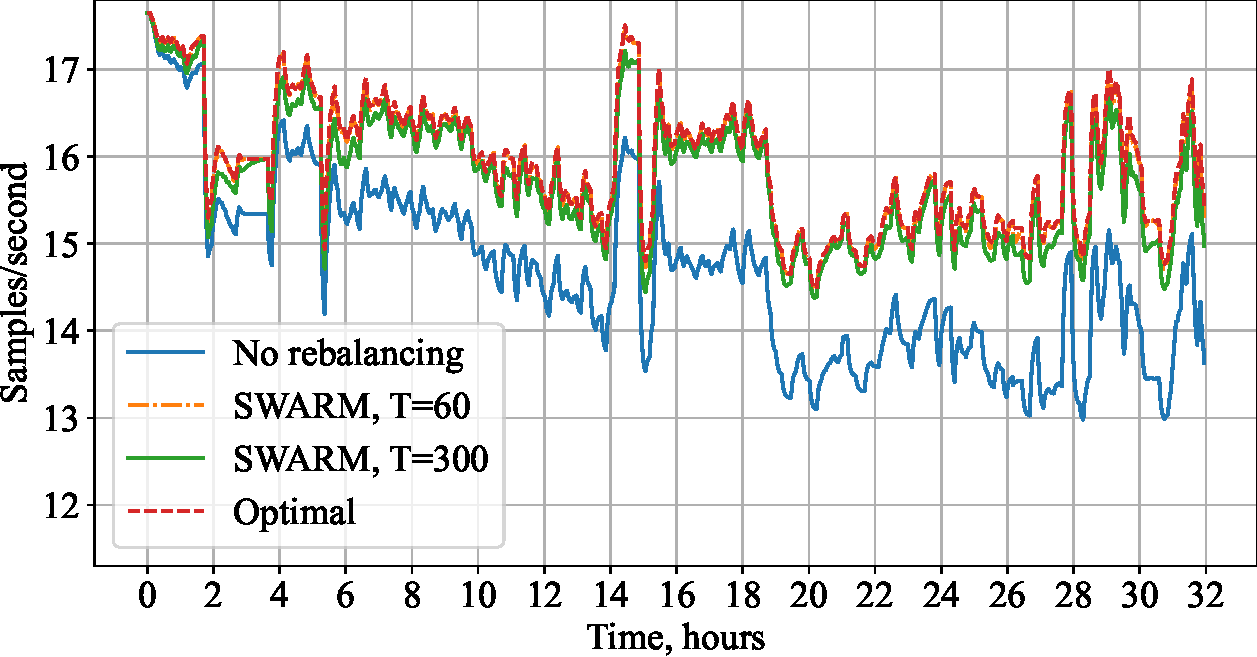
\includegraphics[width=\linewidth]{resources/rebalancing_activity.pdf}
    \captionof{figure}{Throughput of rebalancing methods over time.}
    \label{fig:rebalancing}
\end{figure}

\subsection{Adaptive Rebalancing Evaluation}


\begin{figure*}[h!]
\begin{subfigure}{0.5\textwidth}
    \centering
    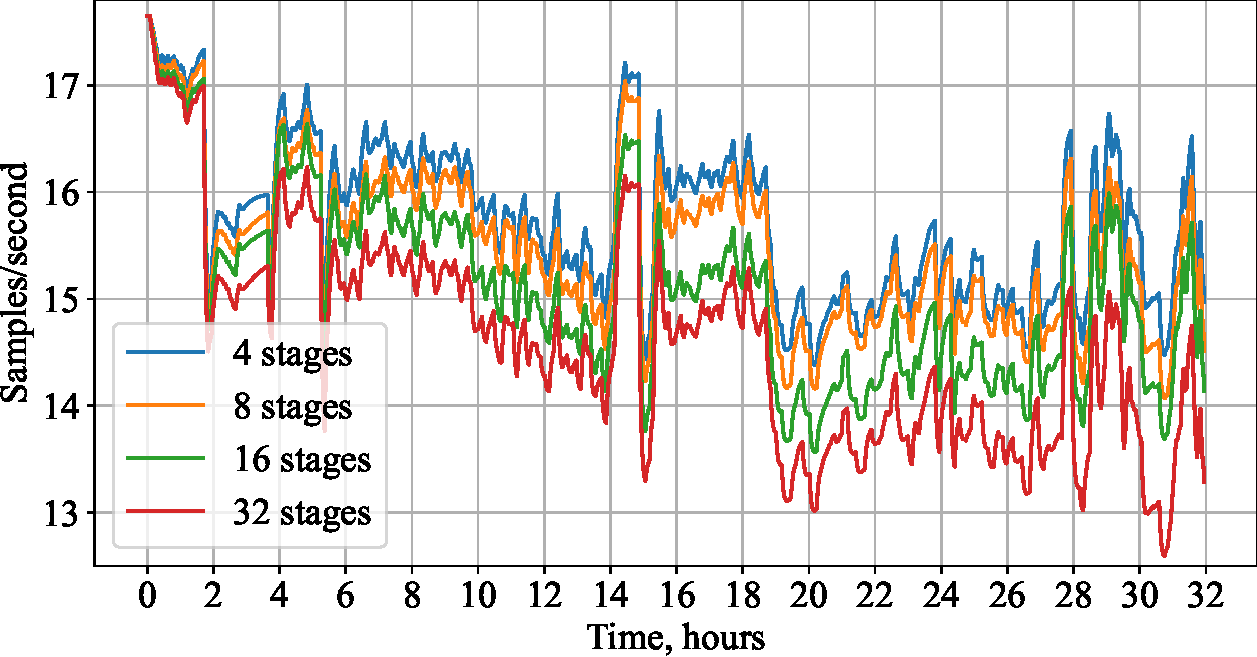
\includegraphics[width=0.97\linewidth]{resources/rebalancing_stages.pdf}
    \caption{Adaptive rebalancing of SWARM parallelism.}
    \label{fig:rebalancing_stages}
\end{subfigure}%
\begin{subfigure}{0.5\textwidth}
    \centering
    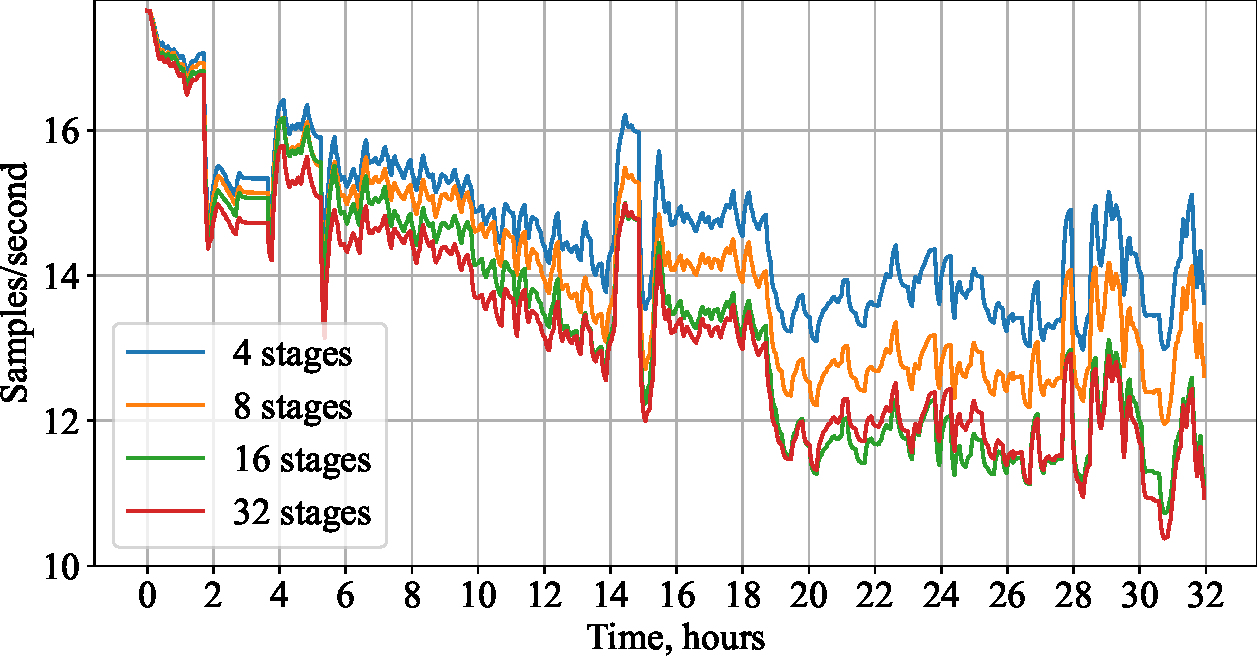
\includegraphics[width=0.97\linewidth]{resources/rebalancing_stages_baseline.pdf}
    \caption{No rebalancing.}
    \label{fig:rebalancing_stages_baseline}
\end{subfigure}
\caption{Scaling of pipeline-parallel strategies with respect to the number of stages.}
\label{fig:rebalancing_stages_all}
\end{figure*}

\label{sect:experiments_adaptive}
In this experiment, we evaluate the efficiency of adaptive peer rebalancing between stages proposed in Section~\ref{sect:method_swarm}. 
We use statistics of the number of active T4 nodes from the 32-hour segment of the experiment described in Section~\ref{sect:experiments_large}. 
We use this data to simulate training dynamics by viewing it as sequence of events, each consisting of a timestamp and a change in the number of peers (which can be positive or negative). 
When a worker is removed from the pipeline, we randomly choose the stage it was removed from: that is, removing $N$ peers corresponds to $N$ samples from the uniform distribution over four pipeline stages. 
We run 10 simulations with different random seeds and average the resulting trajectories.
We compare our strategy with two different values of $T$ to the baseline that has no rebalancing.

The results of this evaluation are available in \autoref{fig:rebalancing}; for reference, we also provide the performance of a theoretically optimal rebalancing strategy that maintains the highest possible throughput at every moment. It can be seen that even with the rebalancing period $T=300$, our approach significantly improves the overall throughput of the pipeline. When the number of peers is relatively stable, the rebalanced pipeline also approaches the optimal one in terms of throughput, which shows the efficiency of rebalancing even when moving only one node at a time.

In addition, we observed that for some brief periods, the performance of the unbalanced pipeline exceeded the throughput of the balanced one due to random choice of disconnecting peers (dropping more from the ``overrepresented'' stages affects the imbalanced pipeline less). However, this held true only for $\approx 4.5\%$ of the experiment and was quickly mitigated by adaptive rebalancing.

As expected, decreasing $T$ from 300 to 60 seconds improves both the overall throughput and the speed of convergence to optimal pipeline performance. However, the effect is not as drastic compared to the increase in DHT data transfer volume. This is also demonstrated by \autoref{tab:rebalancing_speedup}, which shows the relative throughput of the three configurations compared to the optimal one. Furthermore, the table displays that while initially there is little difference between rebalancing choices, it becomes more pronounced later on as the imbalanced version ``drifts further'' from the optimal state.

\begin{table}[b]
\centering
\captionof{table}{Relative throughput comparison of pipeline rebalancing methods.}
\small
\label{tab:rebalancing_speedup}
\begin{tabular}[b]{@{}lccc@{}}
\toprule
\multirow{2}[2]{*}{\thead{Rebalancing}} & \multicolumn{3}{c}{\% of optimal} \\ \cmidrule(l){2-4} 
                        & Overall   & First 1 hour   & Last 1 hour  \\ \midrule
None                & 82.7      & 99.0       & 45.4     \\
$T=300$    & 95.8      & 99.4       & 88.9     \\
$T=60$     & 97.6      & 99.8       & 91.7     \\ \bottomrule
\end{tabular}
\end{table}

Finally, we analyze the scaling properties of rebalancing with respect to the number of stages. To do this, we conduct experiments in the same setup as above ($T=300$) while changing the number of pipeline stages from 4 to $\{4,\ 8,\ 16,\ 32\}$. To ensure the consistency of throughput across all experiments, we increase the starting number of peers accordingly while keeping the preemption rate constant. As a baseline, we also evaluate the throughput of the pipeline that has no rebalancing.

Figure~\ref{fig:rebalancing_stages_all} shows the outcome of this experiment. As displayed in the plots, both strategies drop in performance with the increase in the stage count: while all stages should drop in performance equally in expectation, in practice, the variances are too large while the number of peers is relatively too small for the asymptotic properties to take place. This effect results in more outliers (large drops in the number of peers) in the preemption distribution for more stages. Still, rebalancing allows to partially mitigate the issue: while we observe a more consistent downward trend for the baseline strategy, the rebalanced pipeline regains its performance over time and achieves a higher overall throughput.

